\documentclass[12pt]{article}
 \usepackage[margin=1in]{geometry} 
\usepackage{amsmath,amsthm,amssymb,amsfonts}
\usepackage{graphicx}
\usepackage{array}
\newcolumntype{P}[1]{>{\centering\arraybackslash}p{#1}}
\newcommand{\N}{\mathbb{N}}
\newcommand{\Z}{\mathbb{Z}}
 
\newenvironment{problem}[2][Problem]{\begin{trivlist}
\item[\hskip \labelsep {\bfseries #1}\hskip \labelsep {\bfseries #2.}]}{\end{trivlist}}
%If you want to title your bold things something different just make another thing exactly like this but replace "problem" with the name of the thing you want, like theorem or lemma or whatever
 
\begin{document}
 
%\renewcommand{\qedsymbol}{\filledbox}
%Good resources for looking up how to do stuff:
%Binary operators: http://www.access2science.com/latex/Binary.html
%General help: http://en.wikibooks.org/wiki/LaTeX/Mathematics
%Or just google stuff
 
\title{Homework-2 \\ Feature Descriptors,Homographies and RANSAC}
\author{N Dinesh Reddy \\ dnarapur@andrew.cmu.edu }

\newpage

\maketitle

\section{Lucas-Kanade Tracking}

\begin{problem}{1.1}
The matrix $A^T A$ is called the structure tensor or as the second-moment matrix of the image at a point. It summarizes the predominant directions of the gradient in a specific neighbourhood of a point, and the degree to which those directions are coherent. It is given as :\\

$$
\begin{bmatrix}
[ \sum_i I_x (q_i)^2 & \sum_i I_x (q_i) I_y (q_i) \\
 \sum_i I_y (q_i) I_x (q_i) & \sum_i I_y (q_i)^2
\end{bmatrix} ^{-1}
 $$
 This matrix is a 2x2 hessian matrix and is computed using the gradients of the image.
 
 In order for the equation $A \Delta p = b$ to be solvable, $A^T A$ should be invertible, or the eigenvalues satisfy $\lambda_1 > \lambda_2 > 0$. To avoid noise issue, usually $\lambda_2$ is required to not be too small. For this method to work properly , the condition is that $\lambda_1$ and $\lambda_2$ are large wnough and have similar magnitute.  
 
\end{problem}
\begin{problem}{1.2}
Code described in LucasKanadeInverseCompositional.m \\ 
\end{problem}
\begin{problem}{1.3}
Code described in testCarSequence.m \\
The Results of inverse Compositional Tracking of luckas kanade on car sequence:\\
  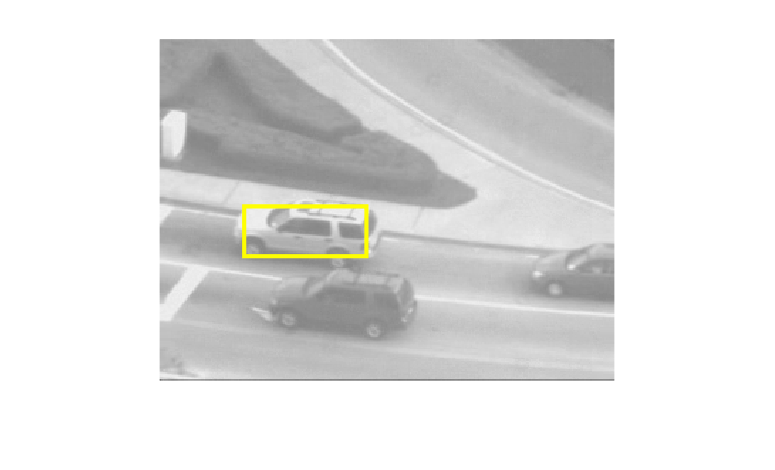
\includegraphics[width=0.21\textwidth]{results/2_car}
  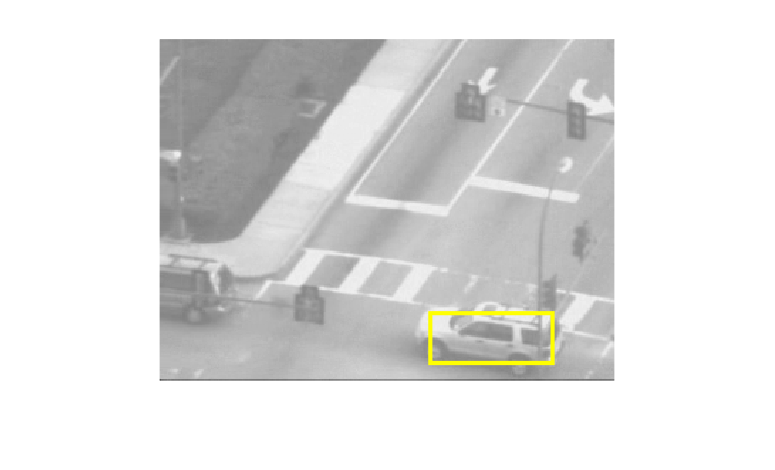
\includegraphics[width=0.21\textwidth]{results/100_car}
  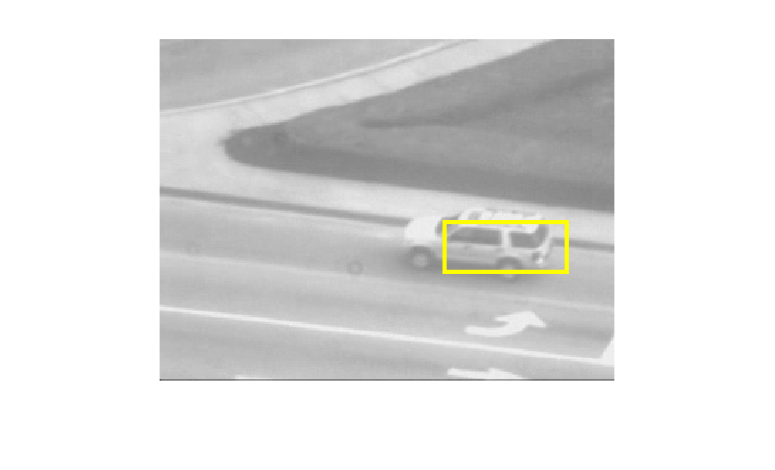
\includegraphics[width=0.21\textwidth]{results/200_car}
  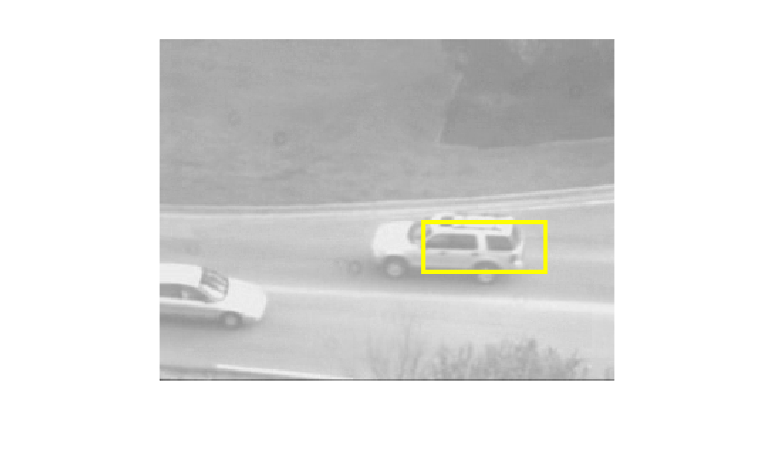
\includegraphics[width=0.21\textwidth]{results/300_car}  
  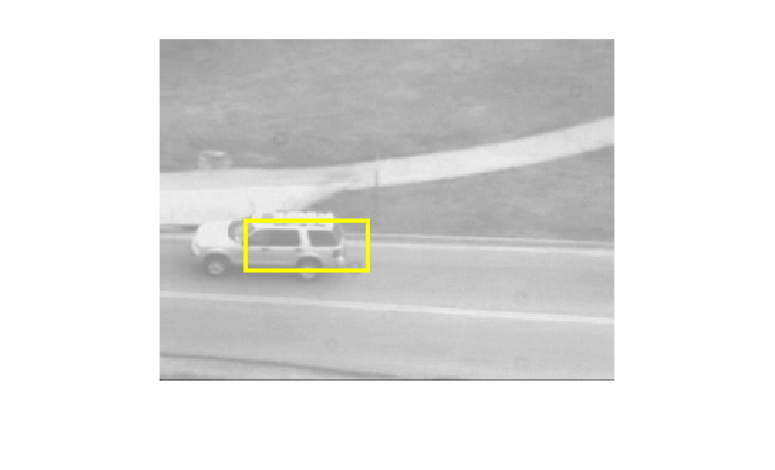
\includegraphics[width=0.21\textwidth]{results/400_car}  
  
The Results of inverse Compositional Tracking of luckas kanade on US sequence:\\

  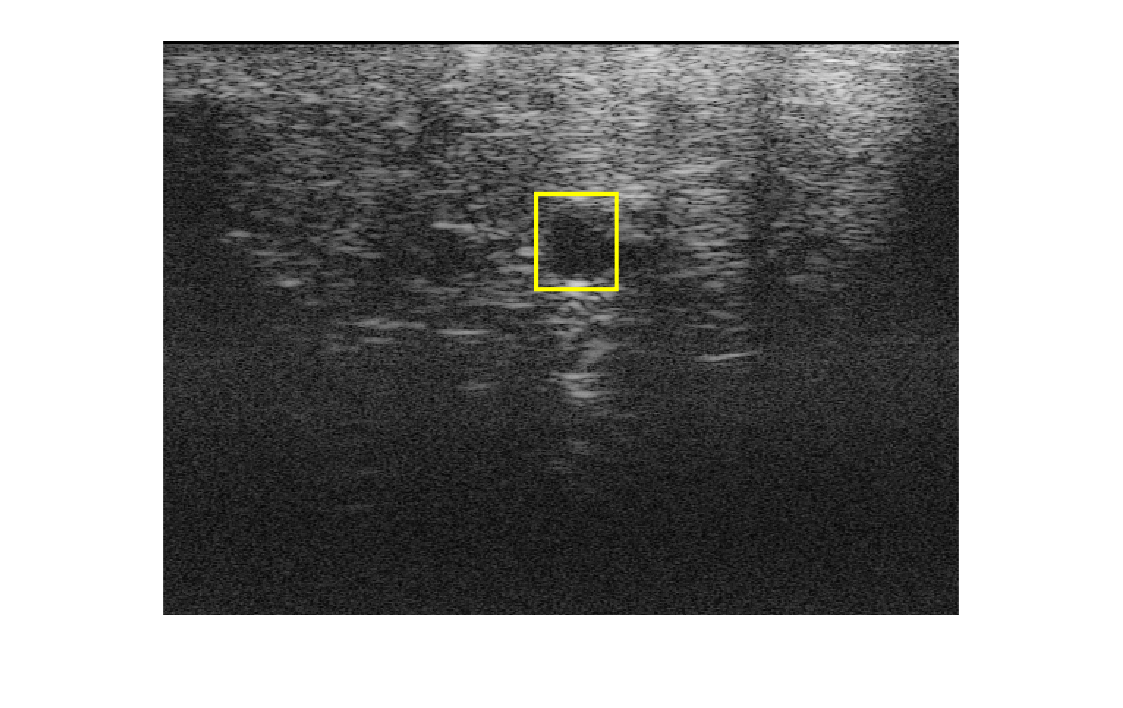
\includegraphics[width=0.21\textwidth]{results/5_us}
  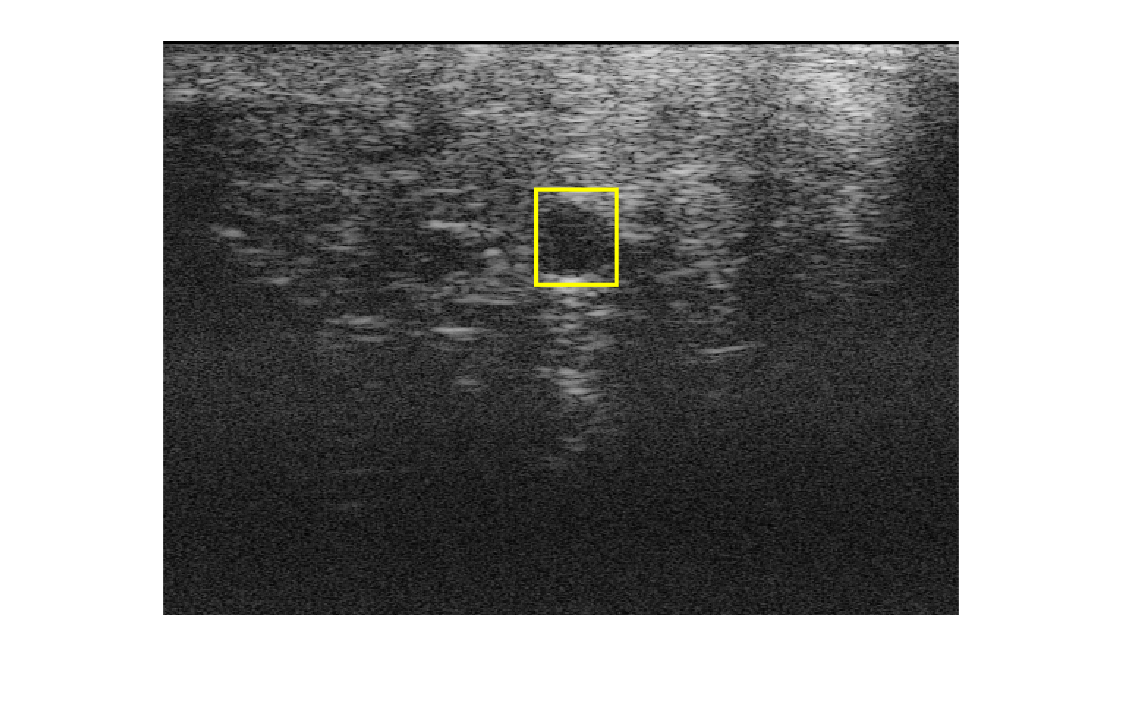
\includegraphics[width=0.21\textwidth]{results/25_us}
  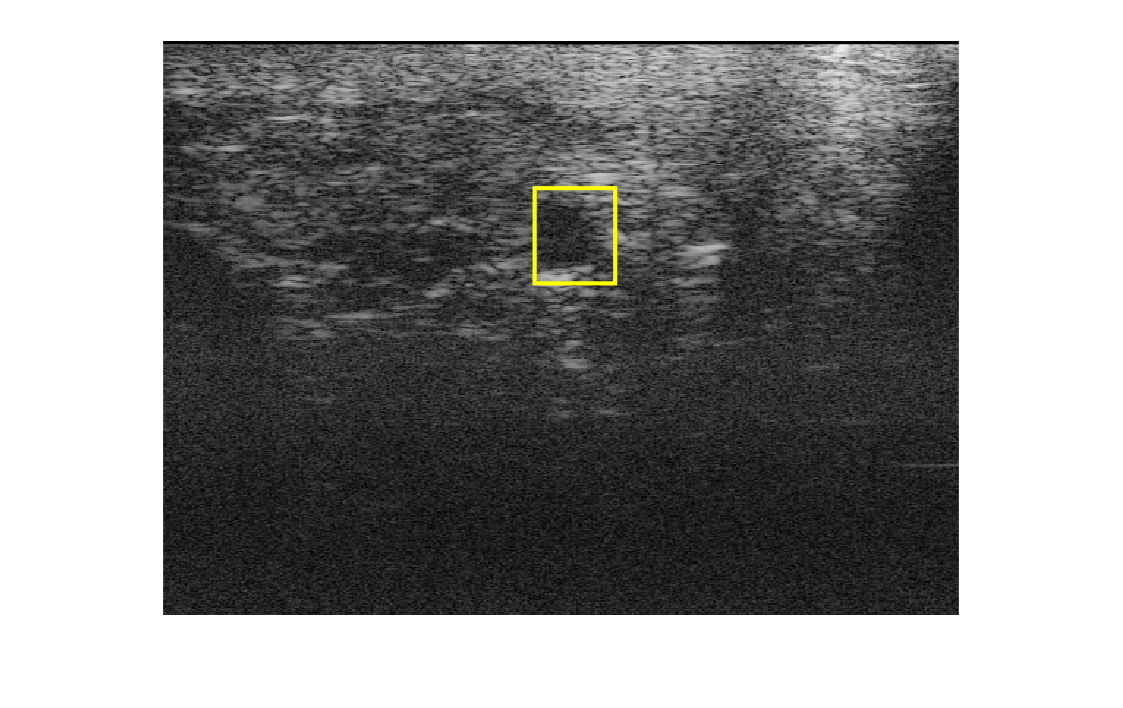
\includegraphics[width=0.21\textwidth]{results/50_us}
  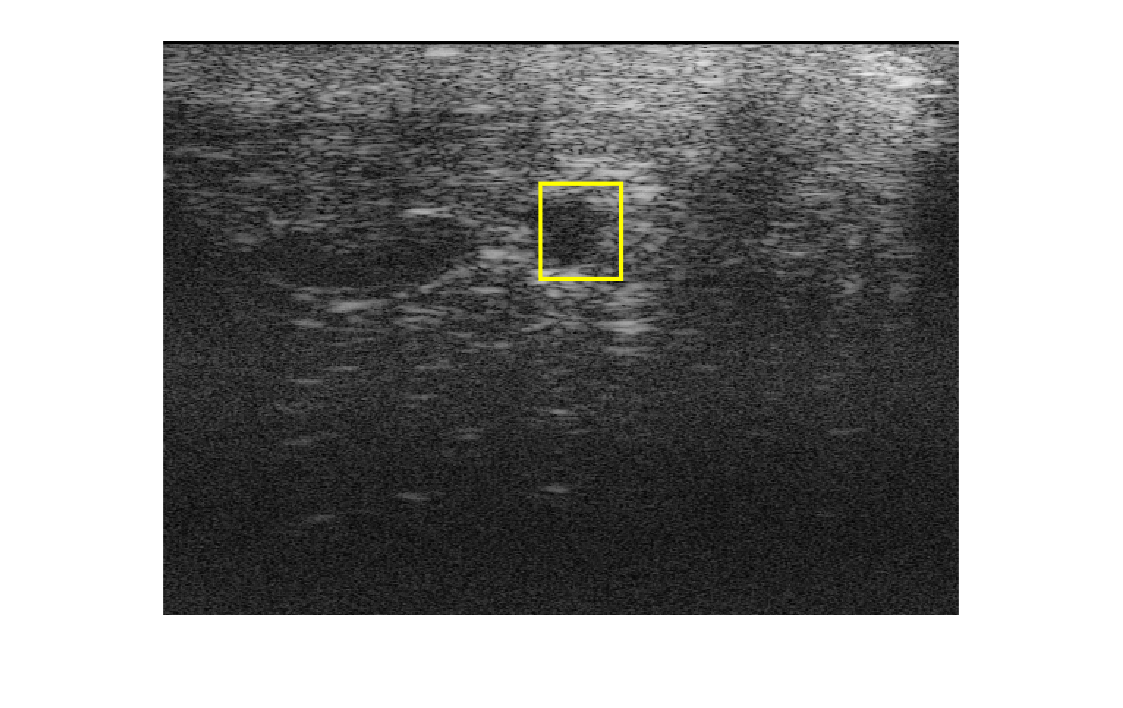
\includegraphics[width=0.21\textwidth]{results/75_us}  
  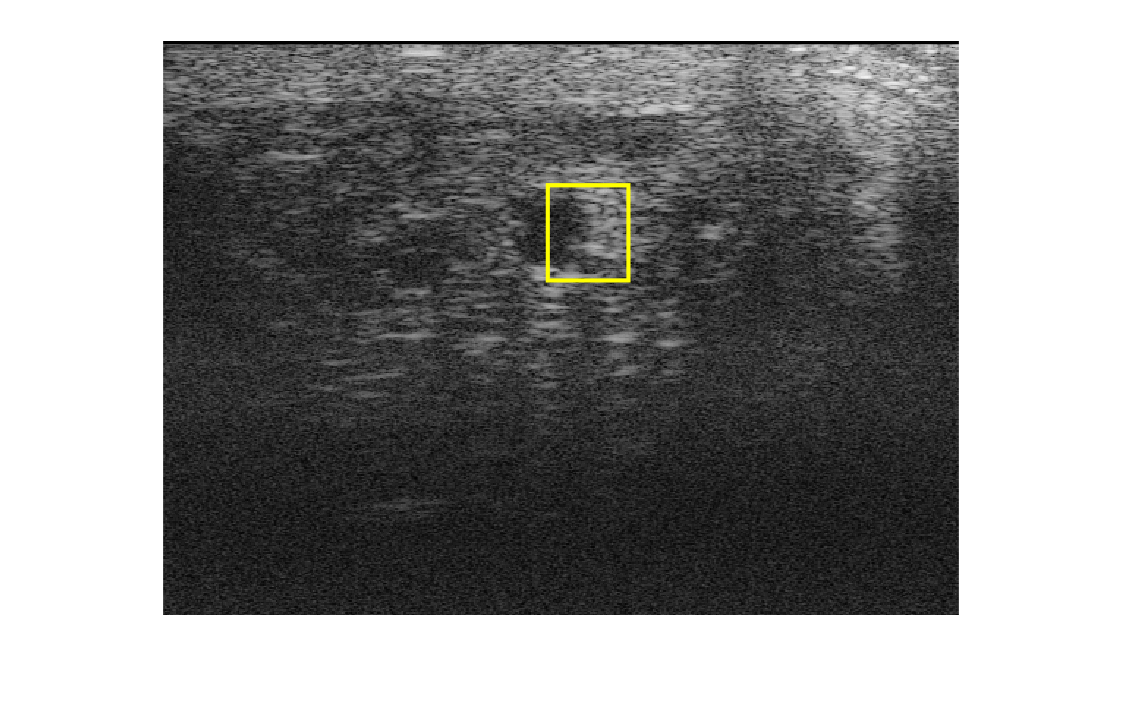
\includegraphics[width=0.21\textwidth]{results/100_us}  

\end{problem}
\begin{problem}{1.4}
We follow the strategy of drift correction proposed by the Ian Matthws et al..
Code described in testCarSequenceWithTemplateCorrection.m and  testUSSequenceWithTemplateCorrection.m\\

The Results of inverse Compositional Tracking of luckas kanade with drift correctionon car sequence:\\
  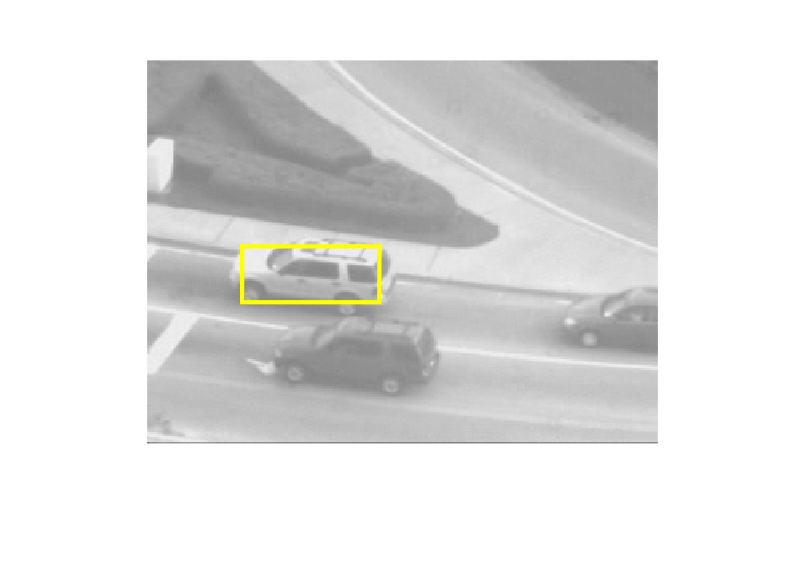
\includegraphics[width=0.21\textwidth]{results/2_car_tempcorr}
  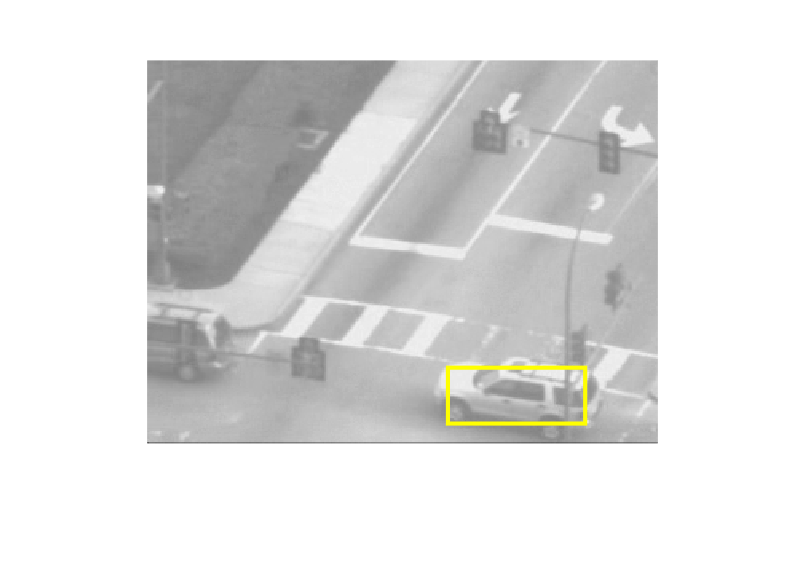
\includegraphics[width=0.21\textwidth]{results/100_car_tempcorr}
  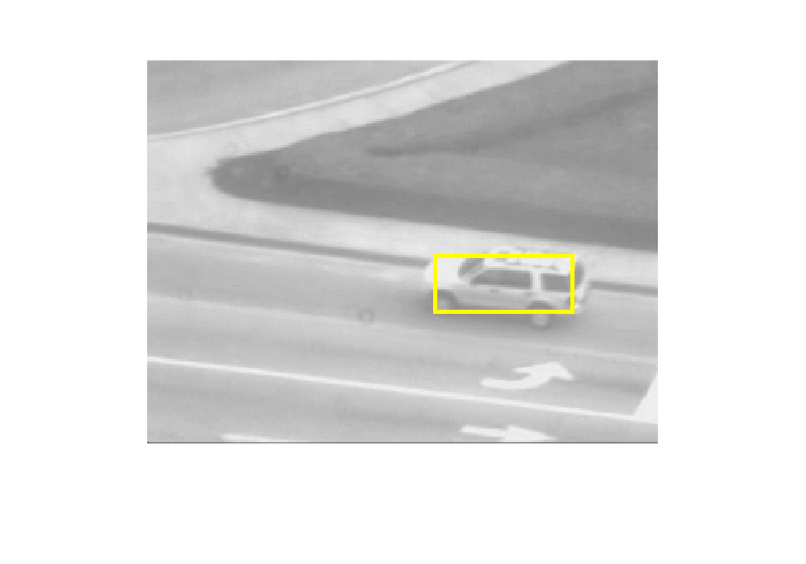
\includegraphics[width=0.21\textwidth]{results/200_car_tempcorr}
  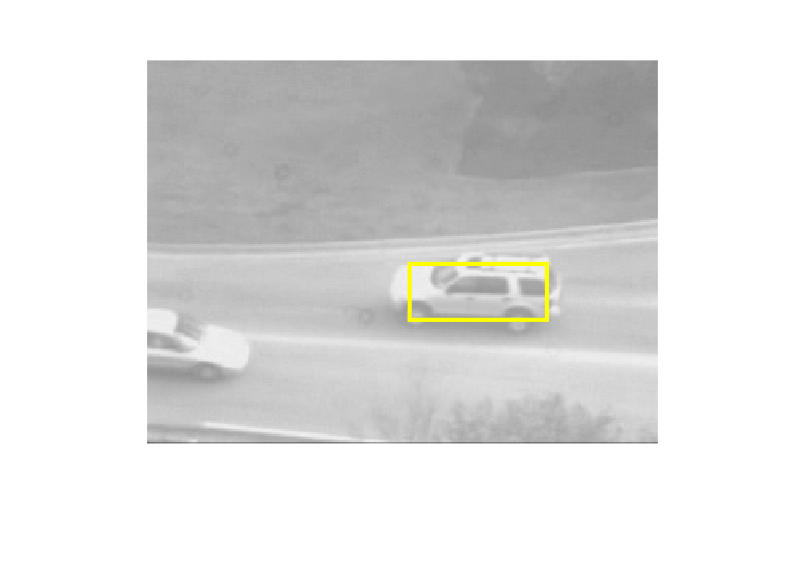
\includegraphics[width=0.21\textwidth]{results/300_car_tempcorr}  
  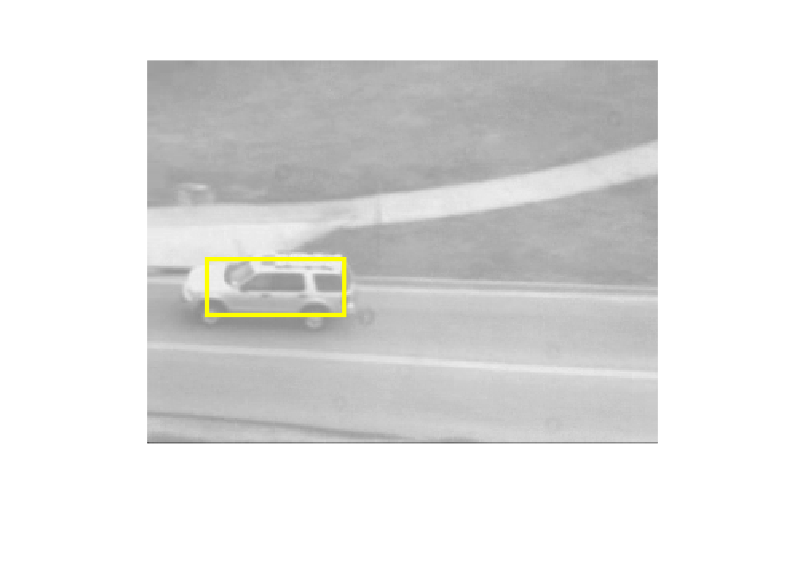
\includegraphics[width=0.21\textwidth]{results/400_car_tempcorr}  
  
The Results of inverse Compositional Tracking of luckas kanade with drift correction on US sequence:\\

  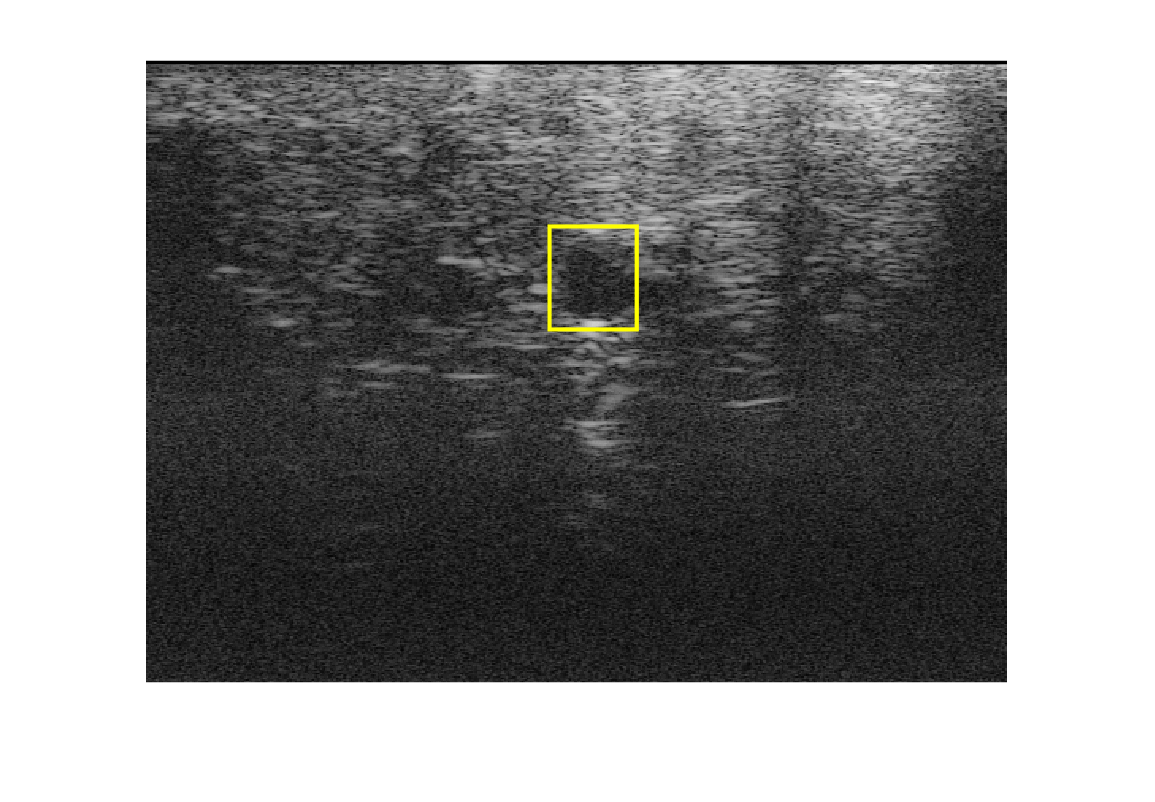
\includegraphics[width=0.21\textwidth]{results/5_us_driftcorr}
  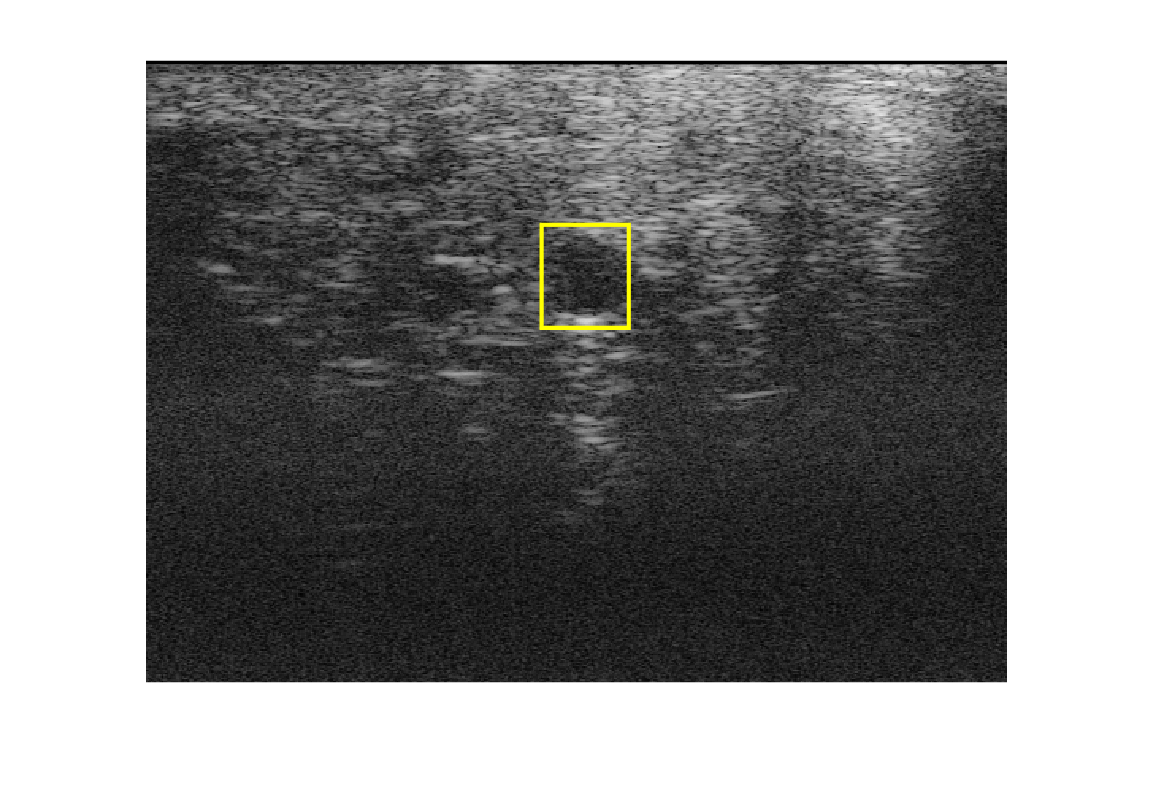
\includegraphics[width=0.21\textwidth]{results/25_us_driftcorr}
  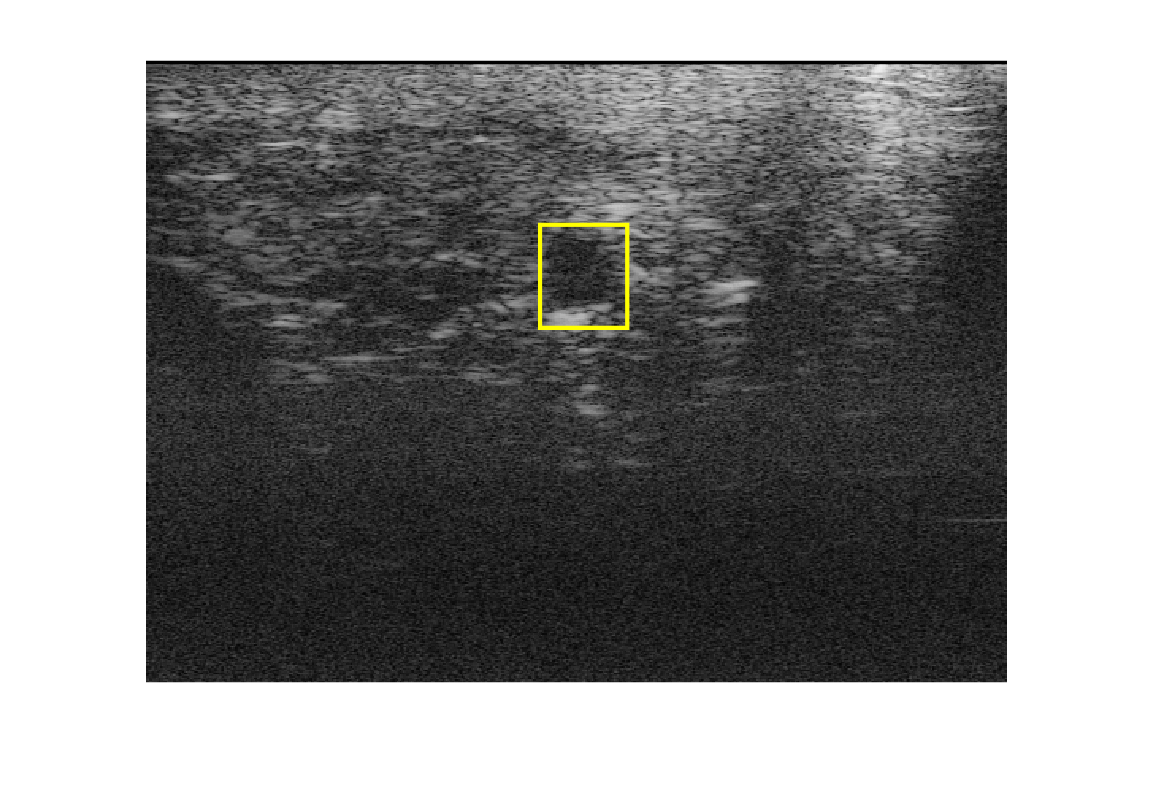
\includegraphics[width=0.21\textwidth]{results/50_us_driftcorr}
  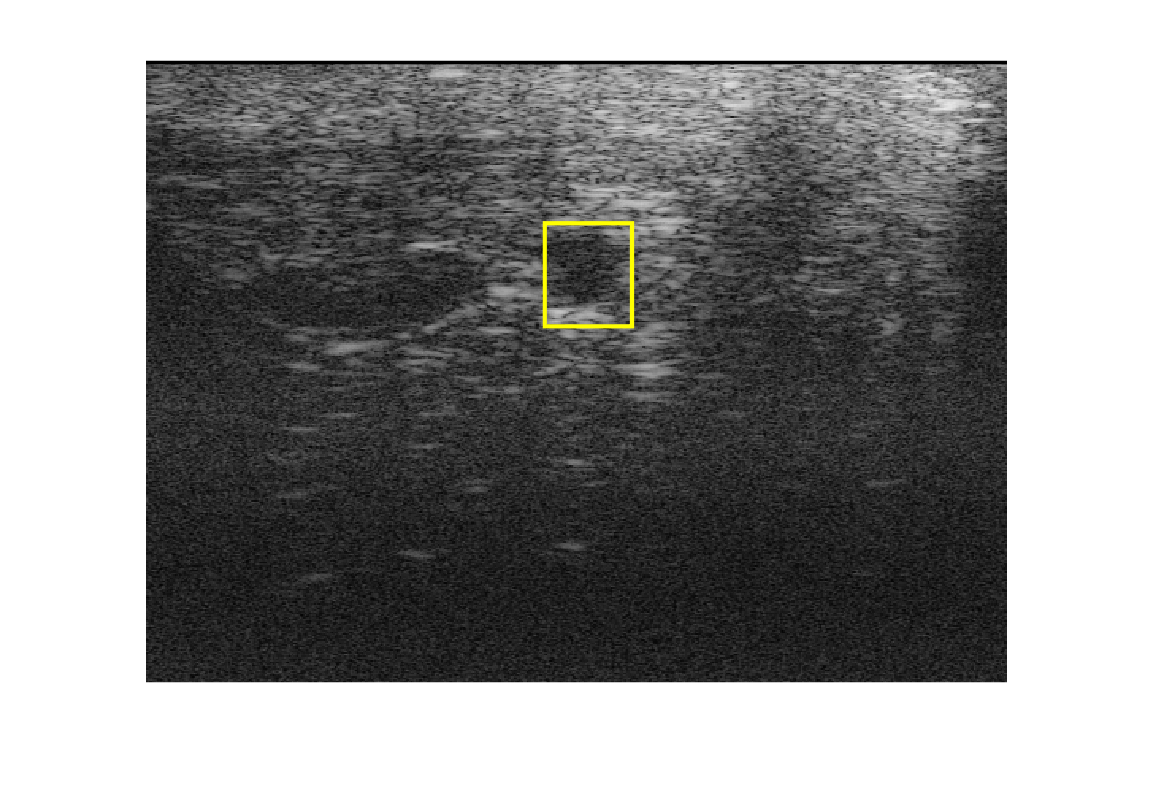
\includegraphics[width=0.21\textwidth]{results/75_us_driftcorr}  
  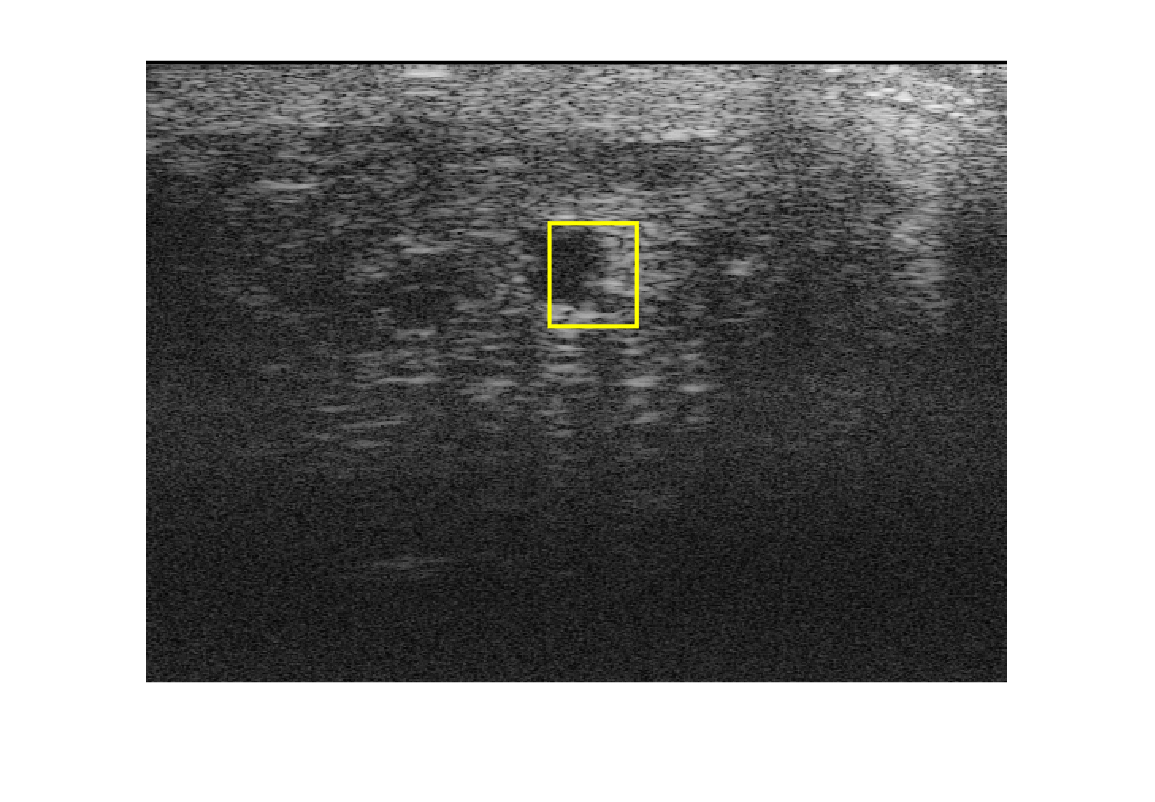
\includegraphics[width=0.21\textwidth]{results/100_us_driftcorr}  

\end{problem}
\newpage
\section{Lucas-Kanade Tracking with Appearance Basis}

\begin{problem}{2.1}

We are given that $I_{t+1} =T_t+ \sum_{c=1..C} w_c B_c$

Since the basic images $B_i$ are othogonal to each other, we multiply both sides by $B_c'$ if we are trying to determine $w_c$.

$$w_c B_c' B_c + \sum_{i=1..C:i \neq c} w_i B_c' B_i = B_c' (I_{t+1}-I_t)$$

$$=> w_c = (B_c' B_c) \backslash (B_c' (I_{t+1}-I_t))$$

The weight vector $w_c$ is essentially discovered as a solution to the optimization problem. 

\end{problem}

\begin{problem}{2.2}
Code described in LucasKanadeBasis.m\\
\end{problem}

\begin{problem}{2.3}
Code described in testSylvSequence.m\\
The Results for the sylv sequence are displayed below:\\
  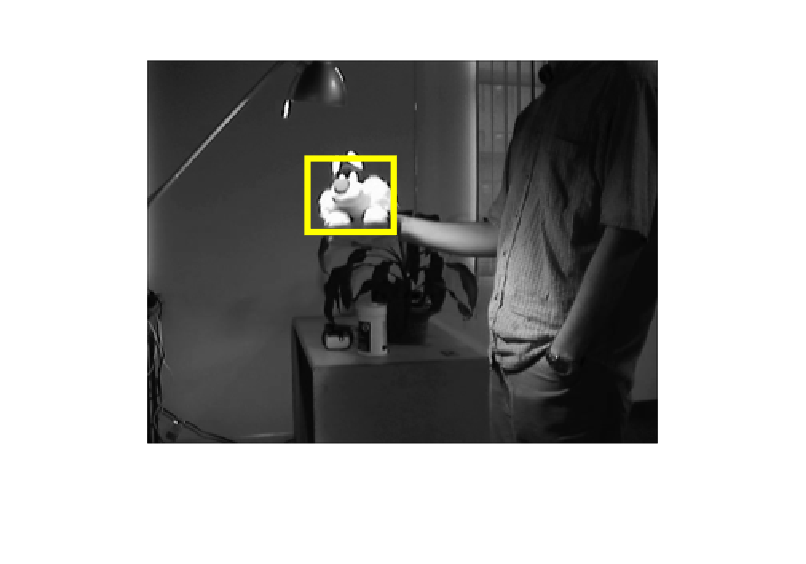
\includegraphics[width=0.21\textwidth]{results/2_sylv}
  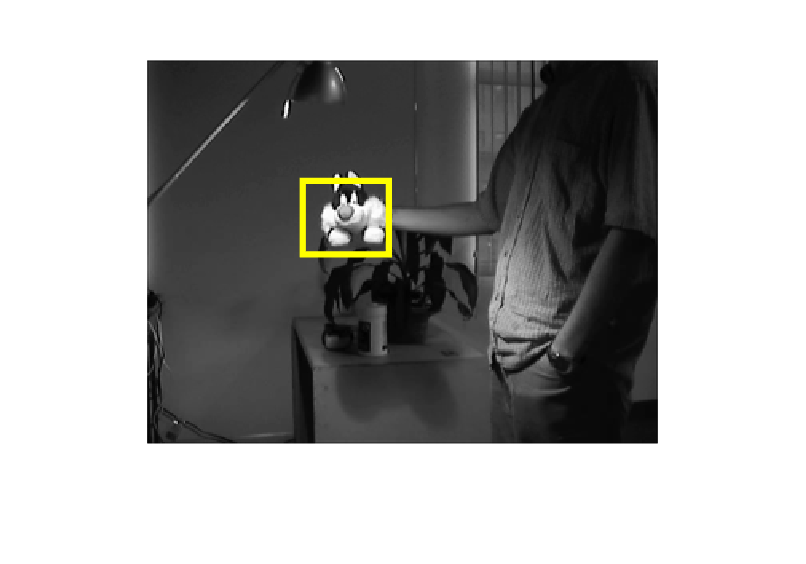
\includegraphics[width=0.21\textwidth]{results/100_sylv}
  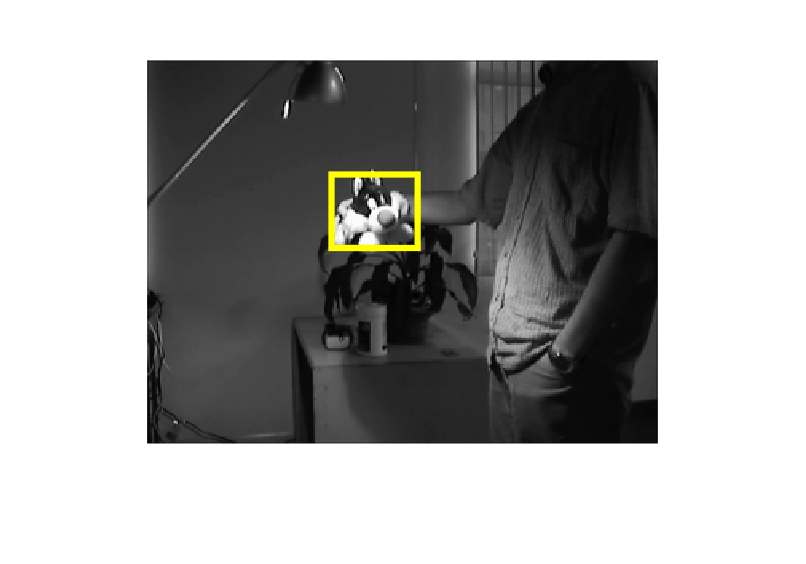
\includegraphics[width=0.21\textwidth]{results/200_sylv}
  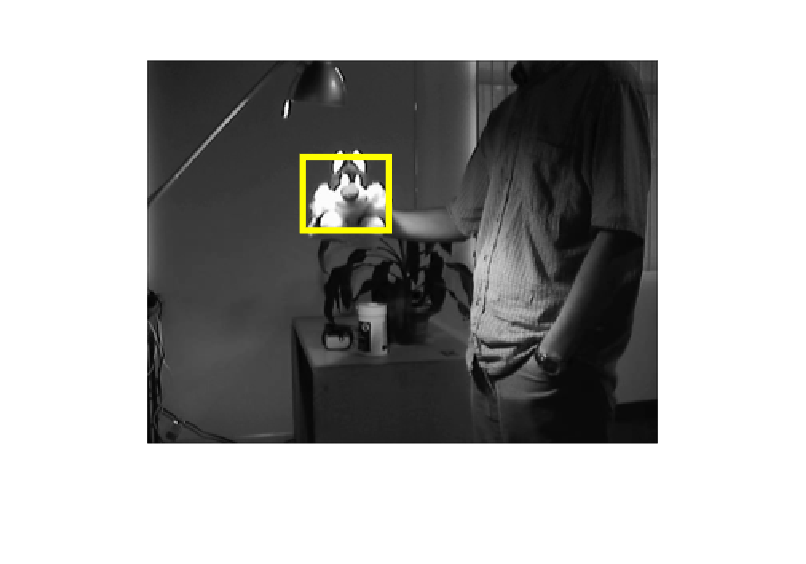
\includegraphics[width=0.21\textwidth]{results/300_sylv}  
  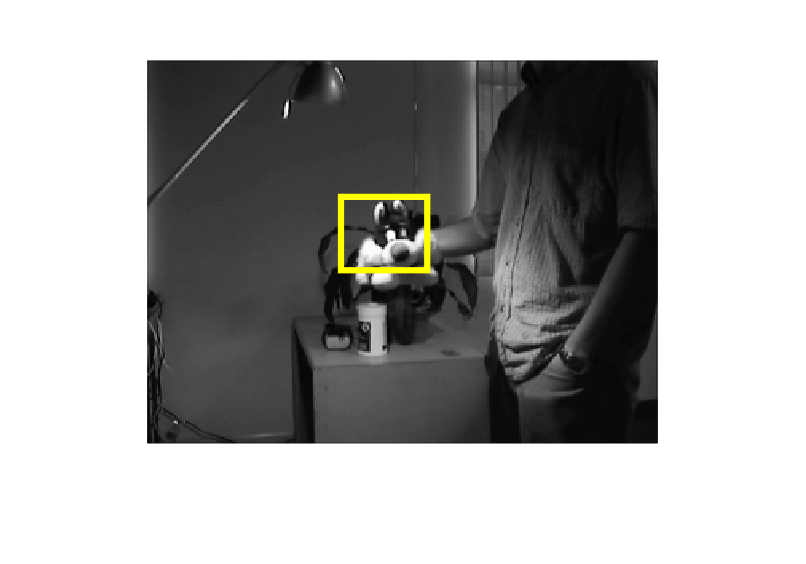
\includegraphics[width=0.21\textwidth]{results/400_sylv}  

\end{problem}

\section{Affine Motion Subtraction}

\begin{problem}{3.1}
Code described in LucasKanadeAffine.m\\
\end{problem} 

\begin{problem}{3.2}
Code described in SubtractDominantMotion.m\\
\end{problem}


\begin{problem}{3.3}
Code described in testAerialSequence.m\\
The results on the aerial sequence using dominant motion subtraction.\\
  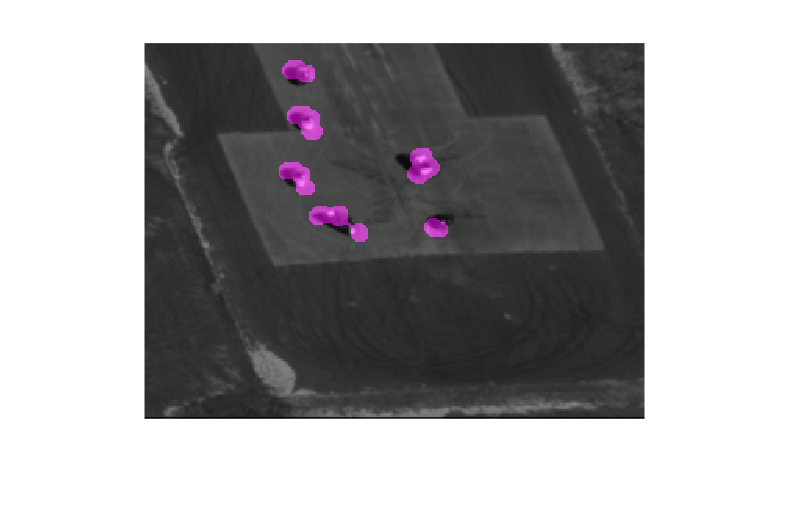
\includegraphics[width=0.27\textwidth]{results/30_ariel}
  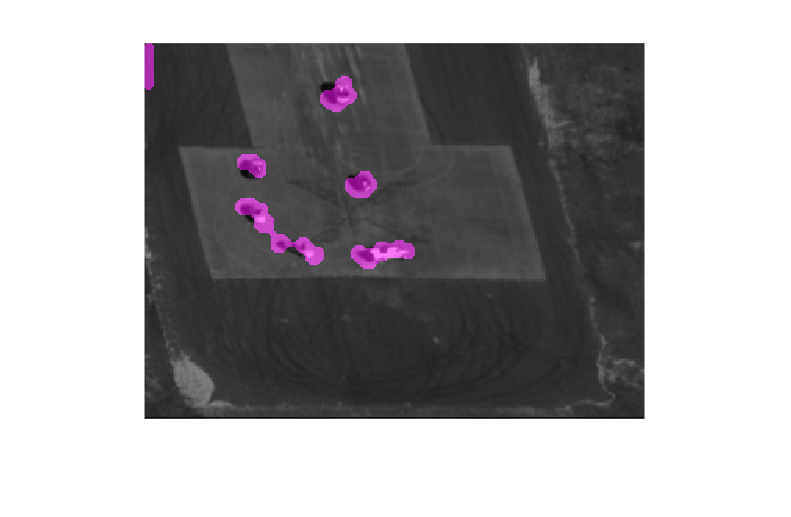
\includegraphics[width=0.27\textwidth]{results/60_ariel}
  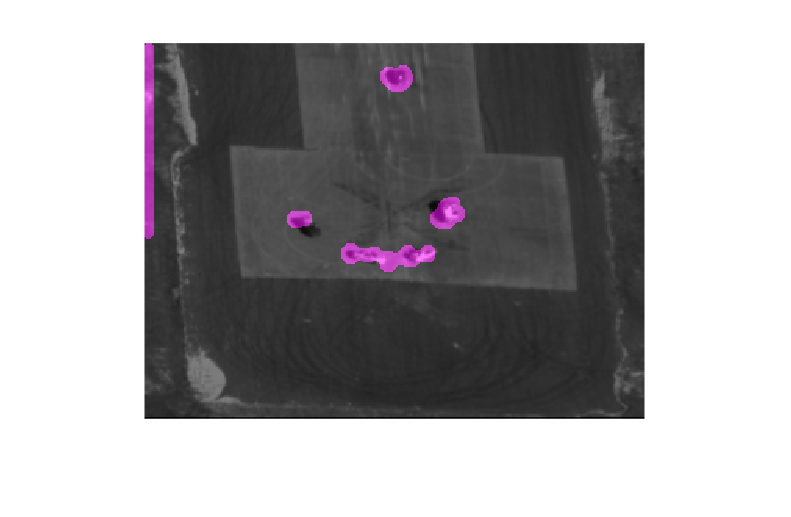
\includegraphics[width=0.27\textwidth]{results/90_ariel}
  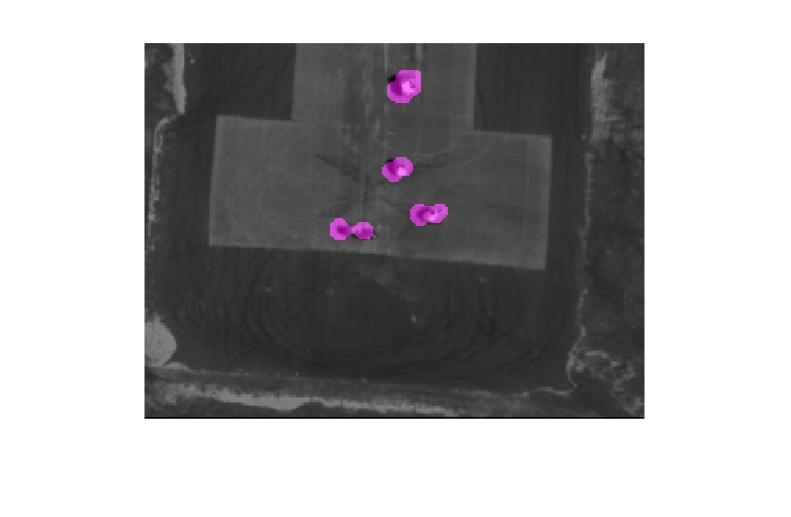
\includegraphics[width=0.27\textwidth]{results/120_ariel}  
\end{problem}


\end{document}